\section{Experiments}
\label{sec:experiments}

In this section, we introduce implementation details, datasets, evaluation metrics. An ablation study of how much each component of the framework contributes and a performance comparison with other supervised or unsupervised methods are also presented.

\subsection{Implementation details.}

Our framework is implemented with publicly available TensorfFlow \cite{abadi2016tensorflow} platform and has 34 million trainable variables in total. During training, Adam optimizer is implemented with parameters $\beta_1 = 0.9$, $\beta_2=0.000$, $\epsilon=10^{-8}$. Learning rate,and batch size are set to be $2\times10^{-3}$ and 4 respectively. Batch normalization \cite{ioffe2015batch} is not used as we didn't observe a performance improvement with it.

The length of input sequence is fixed to be 3 and the input frames are resized to $128 \times 416$. The middle frame is treated as the target image and the other two are source images. With the settings above, the network starts to show meaningful results after 3 epochs of training, and converge at the end of 5th epoch. On a Nvidia Titan X (Pascal) GPU, the training process takes around 6 hours. The number of epochs and absolute time needed for convergence is much less than \cite{godard2016unsupervised} (50 epochs, 25 hours) and \cite{zhou2017unsupervised} (15 epochs).

As the predicted depth is not absolute value but defined up to a scale, we correct the scale factor by enforcing the predicted median matching the ground truth median. That is, multiplying the predicted depth by a factor $\hat{f}$: $\hat{f} = \mathrm{median}(D_{gt}) / \mathrm{median}(D_{pred})$. 

\subsection{Datasets and metrics}
\textbf{Training.}
Theorectically, our framework can be trained on any frame sequences captured with a monocular camera. To better compare with other methods, we evaluate on the popular KITTI 2015 \cite{geiger2012we} dataset. KITTI 2015 dataset is a large dataset suite for multiple tasks, including optical flow, 3D object detection and tracking, semantic segmenations, etc. The raw data of this dataset contains RGB and gray-scale videos, which are captured by stereo cameras from 61 scenes, with a typical image being $1242 \times 375$ in original size.

Videos captured by both left and right cameras are used for training, but treated independently. The same training frame sequences as in \cite{zhou2017unsupervised} are used: training split used by Eigen \etal  \cite{eigen2014depth} excluding frames from test scenes and static sequences. This results in a total of 40,109 trainig sequences and 4431 validation sequences. Different from \cite{godard2016unsupervised}, no other data augmentation has been performed.

\textbf{Testing.} 
There are two splits of KITTI 2015 test data: (1) KITTI split contains 200 high-quality disparity images provided as part of official KITTI training set; (2) Eigen split contains 697 test images proposed by \cite{eigen2014depth}. To better compare with other unsupervised and supervised methods, we present evaluation methods on both two splits. 

The depth ground truth of Eigen split is generated by projecting 3D points scanned from Velodyne laser to the camera view. This produces depth values for less than 5\% of all pixels in the RGB images. To be consistent when comparing with other methods, the same crop as in \cite{eigen2014depth} is implemented when testing. The depth ground truth of KITTI split contains sparse depth map with CAD models in place of moving cars. It provides better quality depth than projected Velodyne laser scanned points but has ambiguous depth value on object boundaries where the CAD model doesn't align with the images. The predicted depth is capped at 80 meters as in \cite{godard2016unsupervised} and \cite{zhou2017unsupervised}.

The normal ground truth for two splits is generated by applying depth-to-normal layer on inpainted depth ground truth. The inpainting algorithm by \cite{silberman2012indoor} has been used. For depth and normal evaluation, only the sparse points with depth ground truth are used.

\textbf{Metrics.} We apply the same depth evaluation and normal evaluation metrics as in \cite{eigen2014depth} and \cite{eigen2015predicting}. For depth evaluation, we use the code provided by~\cite{zhou2017unsupervised} and for normal, we implement ourselves and verified the correctness through evaluating results from \cite{eigen2015predicting}.

% Abs Rel: $\frac{1}{|D|}\sum_{d_{pred}\in D}|d_gt - d_{pred}|/d_gt$

% Sq Rel: $\frac{1}{|D|}\sum_{d_{pred}\in D}||d_gt - d_{pred}||^2/d_gt$

% RMSE: $\sqrt{\frac{1}{|D|}\sum_{d_{pred}\in D}||d_{gt} - d_{pred}||^2}$

% RMSE log: $\sqrt{\frac{1}{|D|}\sum_{d_{pred}\in D}||\log d_{gt} - \log d_{pred}||^2}$

% $\delta<thr$: $\%$ of $d_{pred}\in D$, s.t. $max(\frac{d_gt}{d_{pred}}, \frac{d_{pred}}{d_{gt}})<thr$

% mean: $\frac{1}{|N|}\sum_{n_{pred}\in N}(n_{gt}\cdot n_{pred})$

% median: $median([(n_{gt}\cdot n_{pred})]_{n_{pred} \in N})$

% degree: $\%$ of $n_{pred} \in N$, s.t. $(n_{gt}\cdot n_{pred}) < degree$

\subsection{Ablation study}

An ablation study is conducted to investigate how much each component contributes to the final performance, evaluated on the KITTI split.

\textbf{Depth and normal geometry consistency.} The impact of adding depth-normal consistency is explored by removing normal-to-depth layer in the framework. The inverse warping process introduced in Sec. \ref{chap:warping} takes input image and directly predicted depth map as input. The performance of framework trained without normal-to-depth layer is shown as the row ``Ours (no d-n)" in Tab. \ref{tbl:ablation}. Besides the performance gain after adding depth and normal consistency, the network converges considerably faster compared to without leveraging such consistency: the full network converges after 5 epochs of training and the network without such consistency regularization converges at 15th epoch.

\textbf{Image gradient in smoothness term.} We explore the effectivness of adding image gradient into smoothness term. By setting $\alpha=0$ in the edge-aware smoothness loss, the image gradient has no effect on the weight of smoothness loss. The results of this variant is shown as ``Ours (smooth no gradient)" in Tab. \ref{tbl:ablation}.

\textbf{Image gradient in normal2depth layer.} When setting the $\alpha =0$ in normal-to-depth layer, the normal direction contributes equally to each ``shifted" depth map. With image gradient in normal-to-depth layer, the normal direction will only contribute to those neighboring points $q$ where there is small image gradient between central point $p$ and $q$, \ie the two points most likely lie on the same plane. With such constraint, the depth evaluation performance is better. 

\textbf{Normal smoothness.} We explore the impact of normal smoothness term by evaluating normal performance comparing framework with and without normal smooothness loss term. The visualization results are shown in Tab. \ref{tbl:normal}.

\begin{table*}[]
\centering
\caption{Depth performance of our framework variants on Kitti test split.}
\label{tbl:ablation}
\fontsize{8.5}{9}\selectfont
\bgroup
\def\arraystretch{1.2}
\begin{tabular}{c|c|c|c|c|c|c|c}
\thickhline
\multirow{2}{*}{Methods}  & \multicolumn{4}{c|}{Lower the better} & \multicolumn{3}{c}{Higher the better}                  \\ \cline{2-8} 
                          & Abs Rel  & Sq Rel  & RMSE  & RMSE log & $\delta < 1.25$ & $\delta < 1.25^2$ & $\delta < 1.25^3$ \\ \hline
Ours (no d-n)             & 0.208    & 2.286   & 7.462 & 0.297    & 0.693           & 0.875             & 0.948             \\
Ours (smooth no gradient) & 0.189    & 1.627   & 7.017 & 0.280    & 0.713           & 0.891             & 0.957             \\
Ours (n2d no img grad)    & 0.179    & 1.566   & 7.247 & 0.272    & 0.720           & 0.895             & 0.959             \\
Ours (no normal smooth)   & 0.172    & 1.559   & 6.794 & 0.252    & 0.744           & 0.910             & 0.969             \\ \hline
\end{tabular}
\egroup
\end{table*}

%\textbf{Image gradient matching.} There is no obvious 

\subsection{Comparison with other methods}

To compare with other supervised and unsupervised methods, our framework is evaluated on both KITTI and Eigen split. The depth evaluation results are shown in Tab. \ref{tbl:sota}. Our method outperforms some some supervised \cite{eigen2014depth}, \cite{liu2016learning} and unsupervised methods \cite{zhou2017unsupervised}, \cite{kuznietsov2017semi} and only prior to \cite{godard2016unsupervised} and \cite{kuznietsov2017semi} (supervised). It is worth noting that \cite{kuznietsov2017semi} (supervised) utilizes the depth ground truth and \cite{godard2016unsupervised} takes stereo image pairs as input, which implies the camera motion is known. On Kitti test split, our method outperforms \cite{godard2016unsupervised} on the Sq Rel metric. As Sq Rel metric penalizes large depth error, our method generates depth maps without much outlier depths.

\begin{table*}[]
\centering
\caption{Single view depth test results on Kitti Eigen split (upper part) and Kitti split(lower part). All methods in this table use Kitti dataset for traning and the test result is capped in the range 0-80 meters. Test result on Kitti test split of Zhou et al. 2017 is generated by training the released model on Kitti dataset only}
\label{tbl:sota}
\fontsize{7}{7.5}\selectfont
\bgroup
\def\arraystretch{1.4}
\begin{tabular}{lllllllllll}
\thickhline
\multirow{2}{*}{Method}                                      & \multirow{2}{*}{Test data}                        & \multicolumn{2}{l}{Supervision} & \multicolumn{4}{l}{Lower the better} & \multicolumn{3}{l}{Higher the better}               \\ \cline{3-11} 
                                                             &                                                   & Depth          & Pose           & Abs Rel  & Sq Rel & RMSE  & RMSE log & $\delta < 1.25$ & $\delta<1.25^2$ & $\delta<1.25^3$ \\ \hline
\multicolumn{1}{l|}{Train set mean}                          & \multicolumn{1}{l|}{\multirow{8}{*}{Eigen split}} & \checkmark     &                & 0.403    & 5.530  & 8.709 & 0.403    & 0.593           & 0.776           & 0.878           \\
\multicolumn{1}{l|}{\cite{eigen2014depth} Coarse}            & \multicolumn{1}{l|}{}                             & \checkmark     &                & 0.214    & 1.605  & 6.563 & 0.292    & 0.673           & 0.884           & 0.957           \\
\multicolumn{1}{l|}{\cite{eigen2014depth} Fine}               & \multicolumn{1}{l|}{}                             & \checkmark     &                & 0.203    & 1.548  & 6.307 & 0.282    & 0.702           & 0.890           & 0.958           \\
\multicolumn{1}{l|}{\cite{kuznietsov2017semi} supervised}   & \multicolumn{1}{l|}{}                             & \checkmark     &                & 0.122    & 0.763  & 4.815 & 0.194    & 0.845           & 0.957           & 0.987           \\
\multicolumn{1}{l|}{\cite{kuznietsov2017semi} unsupervised} & \multicolumn{1}{l|}{}                             &                & \checkmark     & 0.308    & 9.367  & 8.700 & 0.367    & 0.752           & 0.904           & 0.952           \\
\multicolumn{1}{l|}{\cite{godard2016unsupervised}}                  & \multicolumn{1}{l|}{}                             &                & \checkmark     & 0.148    & 1.344  & 5.927 & 0.247    & 0.803           & 0.922           & 0.964           \\
\multicolumn{1}{l|}{\cite{zhou2017unsupervised}}                    & \multicolumn{1}{l|}{}                             &                &                & 0.208    & 1.768  & 6.856 & 0.283    & 0.678           & 0.885           & 0.957           \\
\multicolumn{1}{l|}{Ours}                                    & \multicolumn{1}{l|}{}                             &                &                & 0.182    & 1.481  & 6.501 & 0.267    & 0.725           & 0.906           & 0.963           \\ \hline
\multicolumn{1}{l|}{Train set mean}                          & \multicolumn{1}{r|}{\multirow{2}{*}{}}            & \checkmark     &                & 0.398    & 5.519  & 8.632 & 0.405    & 0.587           & 0.764           & 0.880           \\
\multicolumn{1}{l|}{\cite{godard2016unsupervised}}                  & \multicolumn{1}{r|}{}                             &                & \checkmark     & 0.124    & 1.388  & 6.125 & 0.217    & 0.841           & 0.936           & 0.975           \\
\multicolumn{1}{l|}{\cite{Vijayanarasimhan17}}        & \multicolumn{1}{l|}{Kitti split}                  &                &                & -        & -      & -     & 0.340    & -               & -               & -               \\
\multicolumn{1}{l|}{\cite{zhou2017unsupervised}}                    & \multicolumn{1}{l|}{\multirow{2}{*}{}}            &                &                & 0.216    & 2.255  & 7.422 & 0.299    & 0.686           & 0.873           & 0.951           \\
\multicolumn{1}{l|}{Ours}                                    & \multicolumn{1}{l|}{}                             &                &                & 0.1648   & 1.360  & 6.641 & 0.248    & 0.750           & 0.914           & 0.969           \\ \hline
\end{tabular}
\egroup
\end{table*}

Some qualitative depth estimation results are shown in Fig. \ref{fig:examples}.

\begin{figure*}
\centering
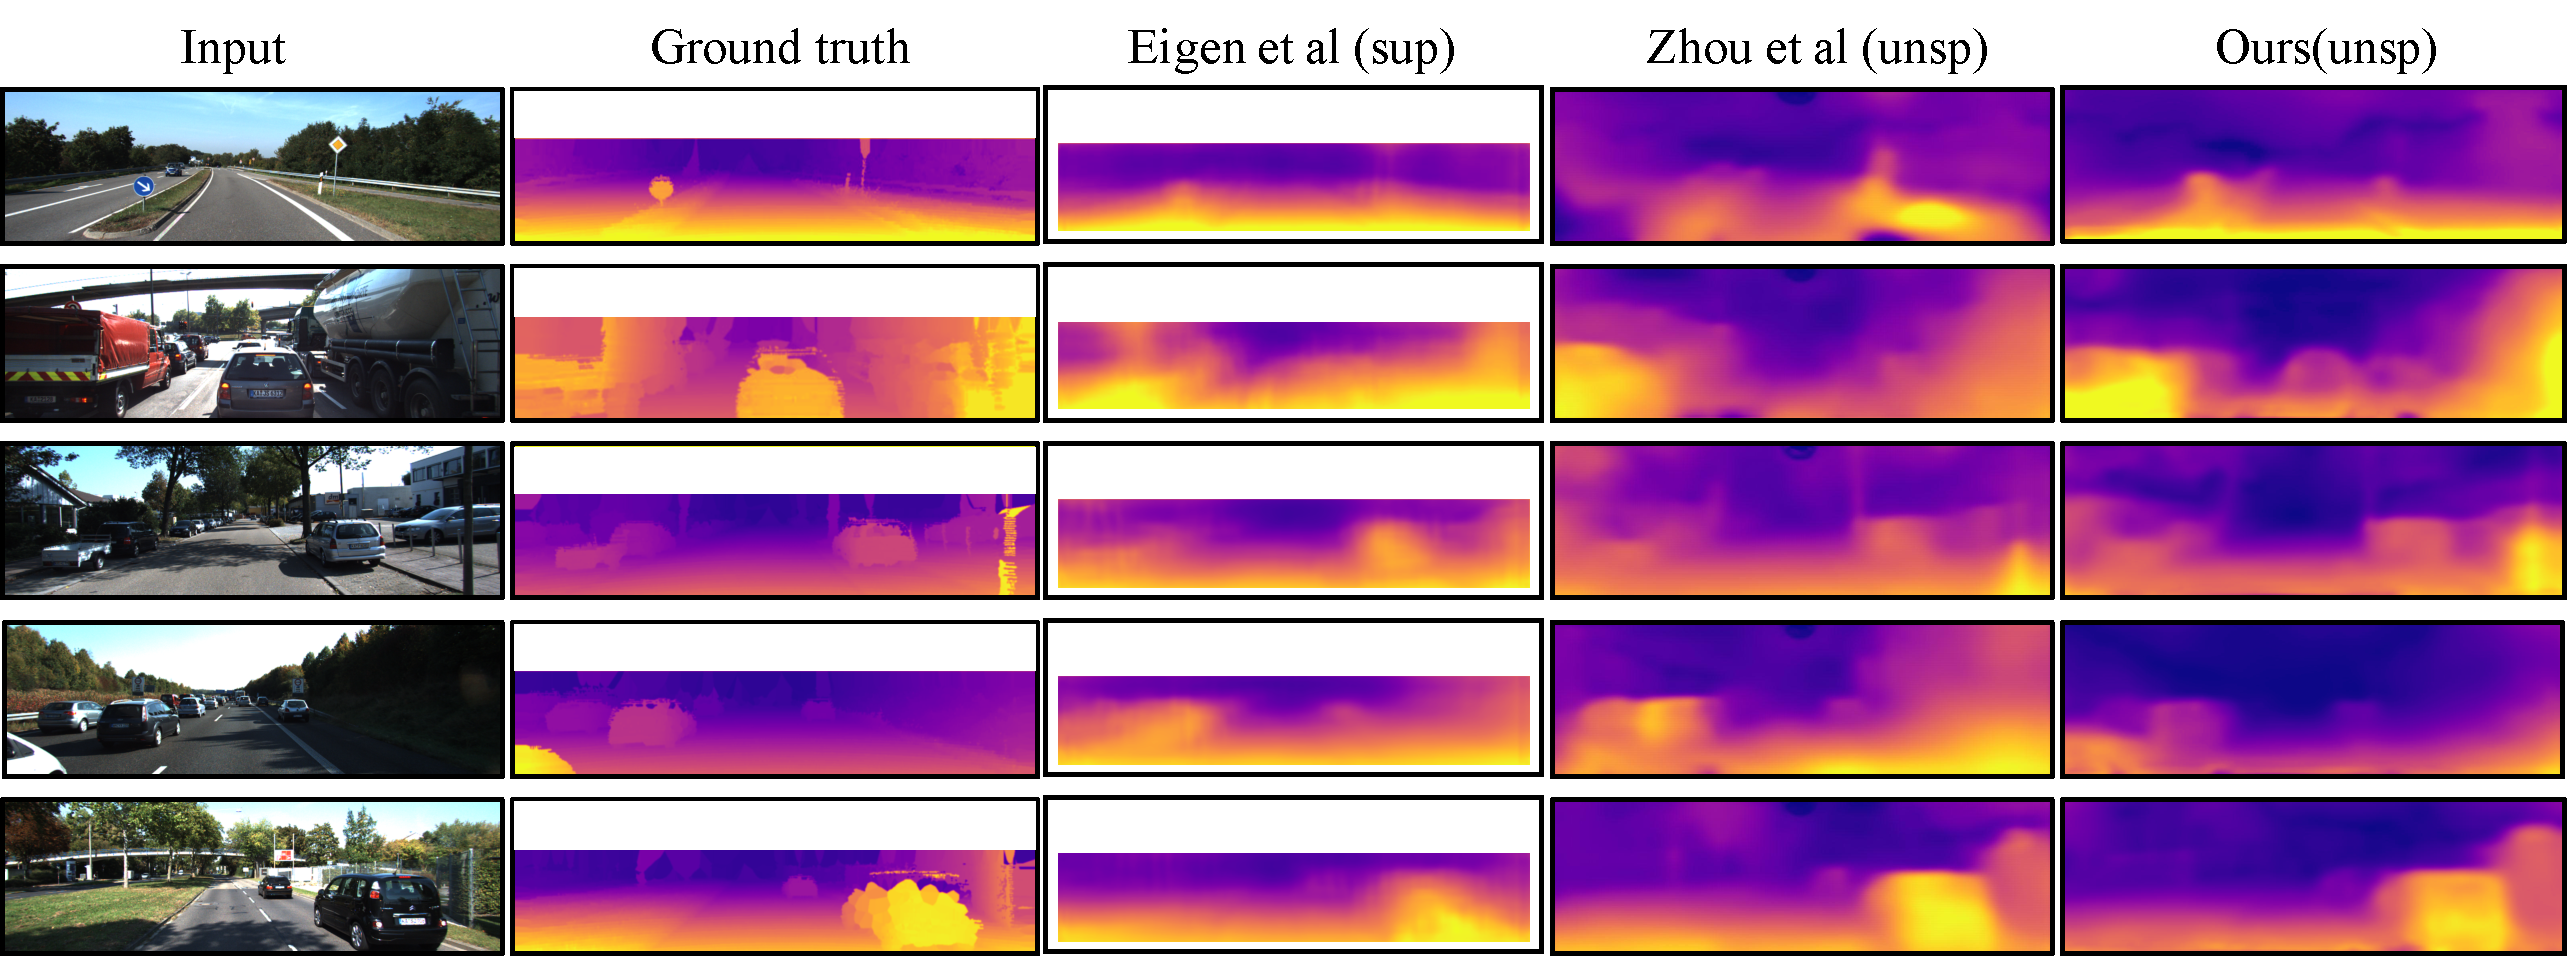
\includegraphics[width=\textwidth]{figures/examples.pdf}
%\caption{1}
\caption{Visual comparison of depth estimation between \protect\cite{eigen2014depth} (supervised with depth ground truth), \protect\cite{zhou2017unsupervised} (unsupervised) and ours (unsupervised). As the original depth ground truth map comes from sparse laser measurement, the interpolated depth map is shown for better visualization.}
\label{fig:examples}
\end{figure*}

To our knowledge, there has not been works that report normal performance on KITTI 2015 dataset. We thus compare our normal performance with baseline methods and normals generated by applying depth-to-normal layer on depth maps of \cite{zhou2017unsupervised}. The baseline methods include ground truth normal mean, normals from pre-defined scene, our framework without second stage training, \ie without normal smoothness term and our full framework. The pre-defined baseline is inspired by by the common scene in Kitti dataset: street plane with walls on both sides. We thus generate a pre-defined normal map based on the scene: 20\% of left and right area of the images are walls and the central 60\% is road.  As shown in Tab. \ref{tbl:normal}, our full model outperforms other baselines under all metrics.

\begin{table}[] \small
\centering
\caption{Normal performances of our method and some baseline methods.}
\label{tbl:normal}
\fontsize{6.5}{7}\selectfont
\bgroup
\def\arraystretch{1.2}
\begin{tabular}{l|c|c|c|c|c}
\thickhline
Method                        & Mean  & Median & $11.25^{\circ}$ & $22.5^{\circ}$  & $30^{\circ}$    \\ \hline
Ground truth normal mean      & 72.39 & 64.72  & 0.031 & 0.134 & 0.243 \\
Pre-defined scene             & 63.52 & 58.93  & 0.067 & 0.196 & 0.302 \\
\cite{zhou2017unsupervised} & 50.47 & 39.16  & 0.125 & 0.303 & 0.425 \\
Ours w/o normal smoothness    & 49.30 & 36.83  & 0.138 & 0.343 & 0.436 \\
Ours                          & 47.52 & 33.98  & 0.149 & 0.369 & 0.473 \\ \hline
\end{tabular}
\egroup
\end{table}

\section{Indoor scene exploration}

Besides the outdoor dataset, we also directly apply our framework on indoor dataset: NYU v2 dataset \cite{silberman2012indoor}. We pick a subset for the preliminary experiment. All training and testing data in NYU dataset related to the scene ``study room" are picked for training and testing in our experiment. As shown in the Fig. \ref{fig:nyu_visual}, our framework performs reasonablly good on scenes that have multiple intersecting planes, but may fail on scenes that have only one object.

\begin{figure}
\centering
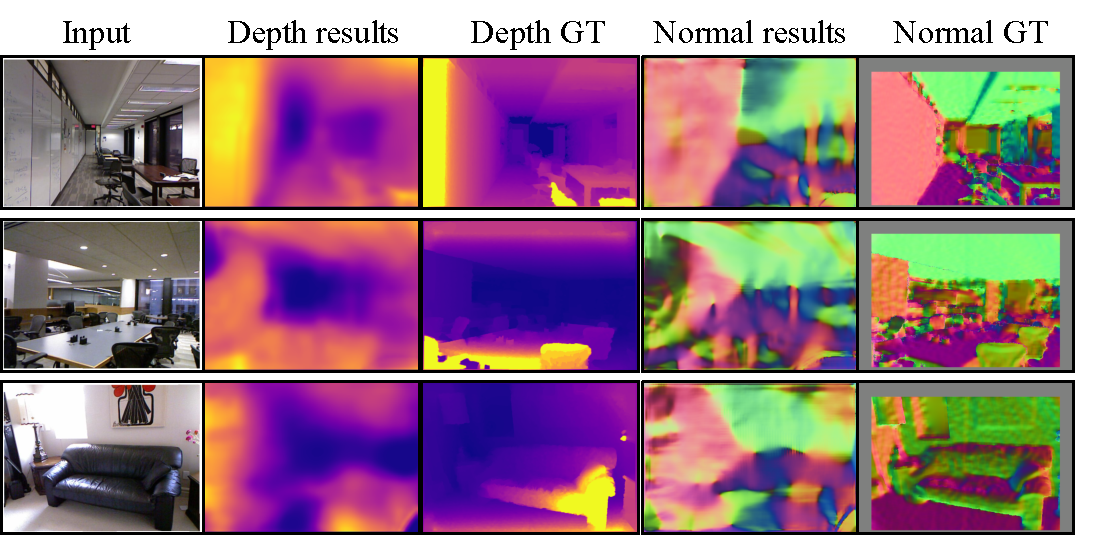
\includegraphics[width=0.5\textwidth]{figures/indoor_visual.pdf}
%\caption{1}
\caption{Qualitative results of our framework on a subset of NYU v2 dataset.}
\label{fig:nyu_visual}
\end{figure}
